\documentclass[czech,a4paper,12pt]{article}[]

\usepackage[nottoc,numbib]{tocbibind}
\usepackage{myDocument, pdflscape, adjustbox,fancyvrb}
\usetikzlibrary{positioning, automata, calc}
\tikzstyle{accepting}=[path picture={%
  \draw let 
    \p1 = (path picture bounding box.east),
    \p2 = (path picture bounding box.center)
    in
      (\p2) circle (\x1 - \x2 - 2pt);
  }]

\lstset{xleftmargin=.3\textwidth, xrightmargin=.3\textwidth}
\renewcommand{\lstlistingname}{Kód}
\setlist{nosep}
\begin{document}
\begin{center}
\LARGE{Vysoké učení technické v Brně \\
Fakulta informačních technologií}
\vfill 
\LARGE{Dokumentace projektu z předmětu IFJ a IAL}\\
\Huge{\textbf{Implementace překladače jazyka IFJ20}}\\
\vfill
\large{\textbf{Tým 101, varianta I}\\
\begin{tabular}{ r l c}
\textbf{Jakšík, Aleš} & \textbf{(\texttt{xjaksi01})} & \textbf{25\%} \\ 
Vlasáková, Nela & (\texttt{xvlasa14}) & 25\% \\  
Mráz, Filip & (\texttt{xmrazf00}) & 25\% \\
Bělohlávek, Jan & (\texttt{xbeloh08}) & 25\% 
\end{tabular}
}\\[3em]
5. 12. 2020
\end{center}

\newpage

\tableofcontents

\newpage

\section{Úvod}
Zadáním projektu bylo vytvořit překladač imperativního jazyka IFJ20 a na jeho vytvoření se podíleli všichni členové týmu. Naživo jsme se viděli jen jednou, pravidelně jsme však komunikovali pomocí Messengeru a hovory jsme realizovali na společném Discordovém serveru. Práci jsme si rozdělili následovně:

\paragraph{Aleš Jakšík}
\begin{inpar}
Vedoucí týmu dostal na práci syntaktickou a sémantickou analýzu vyjma analýzy výrazů, navíc také implementoval tabulku symbolů.

\medskip
\textbf{Soubory:}
    \begin{itemize}
    \item \texttt{parser.c/parser.h}
    \item \texttt{symtable.c/symtable.h}
\end{itemize}
\end{inpar}

\paragraph{Nela Vlasáková}
\begin{inpar}
Na práci dostala syntaktickou a sémantickou analýzu výrazů, k čemuž patří i implementace obousměrně vázaného seznamu, dokumentaci a testování kódu.

\medskip
\textbf{Soubory:}
\begin{itemize}
    \item \texttt{expression.c/expression.h}
    \item \texttt{exprList.c/exprList.h}
\end{itemize}
\end{inpar}    

\paragraph{Filip Mráz}
\begin{inpar}
Na starost dostal generování výsledného kódu a implementaci dynamického řetězce, dále se podílel na implementaci obousměrně vázaného seznamu pro lexikální analyzátor.

\medskip
\textbf{Soubory:}
\begin{itemize}
    \item \texttt{generator.c/generator.h}
    \item \texttt{tokenList.c/tokenList.h}
    \item \texttt{dynamicString.c/dynamicString.h}
\end{itemize}
\end{inpar}

\paragraph{Jan Bělohlávek}
\begin{inpar}
Honzovým úkolem bylo vytvořit lexikální analyzátor, pro který také vytvořil konečný automat.

\medskip
\textbf{Soubory:}
\begin{itemize}
    \item \texttt{scanner.c/scanner.h}
\end{itemize}
\end{inpar}

\newpage
\section{Návrh}
Celý překladač je složen z několika spolupracujících modulů. Každý má většinou jednu hlavní funkci, která je z jiného modulu volána, a tak tedy dojde k jakési komunikaci a předání informací. Kromě vrácení návratové hodnoty mohou takové funkce také zapisovat do různých proměnných (pomocí předání ukazatele na danou proměnnou), a oznamovat tak jiným modulům různé skutečnosti, příkladem by mohlo být například získání datového typu výrazu. Chybová návratová hodnota je předávána vždy zpět od místa, kde se vyskytla, až do \texttt{main.c}, kde je vyhodnocena, je na standartní chybový výstup vytištěna chybová hláška a program je ukončen s touto předávanou hodnotou.

\smallskip
K implementaci jsme využili dvou datových struktur - \textbf{binárního stromu} (pro tabulku symbolů) a \textbf{oboustranně vázaného seznamu}, který je používán jak pro nahrání celého vstupního souboru, tak například pro předávání výrazů k analýze, nebo následně předání výrazu ve formě postfixu k tištění. 

\smallskip
Pro lexikální analýzu jsme využili \textbf{konečného automatu}, při syntaktické kontrole jsme využili LL-gramatiky a \textbf{metody rekurzivního sestupu}. Výrazy jsme zpracovali podle \textbf{precedenční syntaktické analýzy}.


\section{Implementace}
Jako první je ze souboru \texttt{main.c} volán syntaktický/sémantický analyzátor - \texttt{parser.c}. Ten si zavolá lexikální analyzátor (jde tedy o syntaxí řízený překlad), který projde celý vstupní soubor, provede lexikální analýzu podle konečného automatu a vytvoří obousměrně vázaný seznam S tzv. \emph{Tokeny} [Kód \ref{tokenCode}]. 

\begin{figure}[h!]
    \begin{lstlisting}[language=C, caption={Implementace struktury tokenu},label=tokenCode, captionpos=b]
typedef struct Token {
    TokenType t_type;
    tStr *atribute;
    struct Token *lptr;
    struct Token *rptr;
} *TokenPtr;
    \end{lstlisting}
\end{figure}

Tento seznam pak předá zpět syntaktickému/sémantickému analyzátoru, který jej projde a provede syntaktickou kontrolu podle LL gramatiky, následně pak zkontroluje sémantiku. Pokud narazí na místo, kde by se měl nacházet výraz, vytvoří z něj další obousměrně vázaný seznam a pošle jej na precedenční analýzu do \texttt{expression.c}, kde je výraz zkontrolován jak po sémantické, tak syntaktické stránce, a v případě, že je vše v pořádku, je vstupní seznam reprezentující výraz převeden na postfix a odeslán dále do generátoru výstupního kódu.

\newpage


\subsection{Lexikální analýza - \texttt{scanner.c}}
Lexikální analýza je řízena konečným automatem [Obrázek \ref{KA}]. Ze vstupu načte vždy jeden znak a postupně je přidává do předem připraveného řetězce, dokud nedojde do stavu, kdy může tento řetězec přijmout nebo zamítnout. Pokud jej může přijmout, vytvoří z něj \emph{Token} a přidá jej do obousměrně vázaného seznamu, který poté, co narazí na \texttt{EOF} (v místě, kde \texttt{EOF} může podle automatu přijít), považuje soubor za lexikálně korektní a předá jej zpět do \texttt{parser.c}.

\subsubsection{Dynamický řetězec - \texttt{dynamicString.c}} 
Práci s řetězci máme řešenou pomocí implementace vlastního dynamického řetězce. Při inicializaci je alkováno místo o předem dané velikosti \texttt{STRING\_LEN} a při každém přidání nového znaku do takto inicializovaného řetězce se v případě, že místo v paměti již existujícího řetězce není dostačující, zvětší vyhrazený prostor o dalších \texttt{STRING\_LEN}, což je předem vytvořená konstanta o hodnotě 10.

\subsection{Syntaktická a sémantická analýza}
Syntaktická kontrola je řízena pravidly \textbf{LL gramatiky}, informace potřebné k sémantické kontrole (existence proměnných a funkcí, datové typy a podobně) jsou uchovávány v \textbf{tabulce symbolů} implementované pomocí binárního stromu. 


\subsubsection{Syntaktická analýza - \texttt{parser.c}}
Začátkem syntaktické analýzy je kontrola, jestli vstupní soubor obsahuje povinnou hlavičku. Následně se celý seznam, který obsahuje \emph{Tokeny} reprezentující vstupní soubor, projde poprvé. Funkce \texttt{buidInFunc} projde všechny hlavičky funkcí, uloží je do tabulky symbolů spolu s informacemi o vstupních a výstupních parametrech (počet a datový typ). Také zkontroluje, že poslední funkcí je \texttt{main}. Po provedení tohoto prvního běhu se pak celý seznam projde znova a kontrolují se těla jednotlivých funkcí. Tato kontrola se řídí pravidly LL gramatiky [Obrázek \ref{gramatika}].

\subsubsection{Sémantická analýza- \texttt{parser.c}}
Při procházení těly funkcí se do tabulky symbolů nahrávají informace o proměnných. Každé tělo představuje novou tabulku symbolů a postup vytváření tabulek je následující:

\begin{enumerate}
    \item \textbf{Vstup do těla} (funkce, konstrukce \texttt{if}, cyklus)
    \item \textbf{Vytvoří se nová tabulka symbolů} a vloží se do seznamu tabulek symbolů (vždy na první místo)
    \begin{itemize}
        \item Hlavička cyklu je vždy samostatná nová tabulka, tudíž je zaručeno, že v ní lze použít proměnné definované dříve a zároveň, že proměnné definované v hlavičce budou dostupné v jejím těle
    \end{itemize}
    \item \textbf{Odchod z těla} znamená odstranění tabulky ze seznamu tabulek symbolů
\end{enumerate}

Ověření, že nějaká proměnná již byla definována (a případné získání datového typu a podobně), pak vypadá tak, že se první podíváme do tabulky na začátku seznamu, a pokud nic nenajdeme, jdeme hlouběji, dokud ji nenajdeme, v opačném případě pak nastává chyba.
\newpage
\subsubsection{Precedenční analýza výrazů - \texttt{expression.c}}
Hlavní funkcí analyzátoru výrazů je funkce \texttt{parseExp}. Ta obdrží seznam \emph{Tokenů}, podle kterého následně vytvoří vlastní seznam, kde jsou prvky identifikovány podle symbolů precedenční tabulce, kterou je celá precedenční analýza řízena. 

Ta je v kódu implementována jako dvourozměrné pole znaků:

\begin{center}
\catcode`\-=12
\begin{tabular}{| c | p{2.3em} | p{2.3em} | p{2.3em} | p{2.3em} | p{2.3em} | p{2.3em} | p{2.3em} | p{2.3em} | p{2.3em} |}
\hline
    & \multicolumn{9}{ c |}{\texttt{input}} \\\hline
    \multirow{9}{*}{\rotatebox[origin=c]{90}{\texttt{opStack}}} & &\centering\textbf{+} & \centering\textbf{-} & \centering\textbf{*} & \centering\textbf{/} & \centering\textbf{(} & \centering\textbf{)} & \centering\textbf{cmp} & \textbf{\;\;\,\$} \\\cline{2-10}
    & \centering\textbf{+} & \centering R & \centering R & \centering S & \centering S & \centering R & \centering S & \centering R & \;\;\,R\\\cline{2-10}
    & \centering\textbf{-} & \centering R & \centering R & \centering S & \centering S & \centering R & \centering S & \centering R & \;\;\,R\\\cline{2-10}
    & \centering\textbf{*} & \centering R & \centering R & \centering R & \centering R & \centering R & \centering S & \centering R & \;\;\,R\\\cline{2-10}   
    & \centering\textbf{/} & \centering R & \centering R & \centering R & \centering R & \centering R & \centering S & \centering R & \;\;\,R\\\cline{2-10}      
    & \centering\textbf{(} & \centering S & \centering S & \centering S & \centering S & \centering R & \centering S & \centering R & \;\;\,R\\\cline{2-10}   
    & \centering\textbf{)} & \centering S & \centering S & \centering S & \centering S & \centering S & \centering S & \centering S & \;\;\,E\\\cline{2-10}   
    & \centering\textbf{cmp} & \centering R & \centering R & \centering R & \centering R & \centering R & \centering E & \centering R & \;\;\,R\\\cline{2-10}   
    & \centering\textbf{\$} & \centering S & \centering S & \centering S & \centering S & \centering S & \centering S & \centering E & \;\;\,A\\\hline 
\end{tabular}            
\end{center}

Princip pro postup při precedenční analýze (a zároveň systém více seznamů) byl nastudován zde \cite{prectable}. Žádný kód nebyl převzat. Analýza pracuje se třemi seznamy:

\begin{enumerate}
    \item \texttt{input} reprezentující vstupní výraz
    \item \texttt{idStack}, do kterého se vkládají výrazů
    \item \texttt{opStack}, kam jsou vkládány operátory
\end{enumerate} 

\medskip
Proměnná, ať už jde o nějaký identifikátor, číslo, desetinný literál nebo řetězec, je klasifikováno jako \texttt{E} (tedy jako výraz). Pokud při procházení seznamem narazíme na prvek označný jako \texttt{E}, rovnou jej vložíme do příslušného seznamu. Samotný proces precedenční analýzy pak probíhá následovně:

\begin{enumerate}
\item Symbol z precedenční tabulky získáme vždy zadáním "souřadnic":
\begin{quote}
\texttt{precTable[x][y]}
\end{quote}
kde \texttt{x} reprezentuje symbol na konci seznamu \texttt{OpStack} a \texttt{y} reprezentuje symbol, na který se právě díváme ve vstupním seznamu.
\item Pokud dostaneme \texttt{R}, provedeme redukci
\item Pokud dostaneme \texttt{S}, provedeme přesunutí symbolu ze vstupu \texttt{input} na \texttt{opStack}
\item Pokud dostaneme \texttt{A}, kontrolujeme, konečné podmínky přijetí výrazu a pokud projdou v pořádku, výraz převádíme na \emph{postfix}.
\end{enumerate}

Princip převodu z notace \emph{infix} na \emph{postfix} byl nastudován zde \cite{postfix}. Žádný kód nebyl převzat.
\medskip
Redukce je prováděna na základě následujících pravidel:

\begin{center}
\ttfamily{ 
\begin{tabular}{r r l c l l l }
&  & (E) & $\rightarrow$ & E & &\\
E + E & $\rightarrow$ & E &  & E - E & $\rightarrow$ & E \\
E / E & $\rightarrow$ & E & & E * E & $\rightarrow$ & E \\
E < E & $\rightarrow$ & E & & E > E & $\rightarrow$ & E \\
E >= E & $\rightarrow$ & E & & E <= E & $\rightarrow$ & E \\
E == E & $\rightarrow$ & E & & E != E & $\rightarrow$ & E \\
\end{tabular}}
\end{center}


\newpage
\subsection{Generování kódů - \texttt{generator.c}}
\newpage
\section{Konečný automat}
\begin{figure}[h!]
    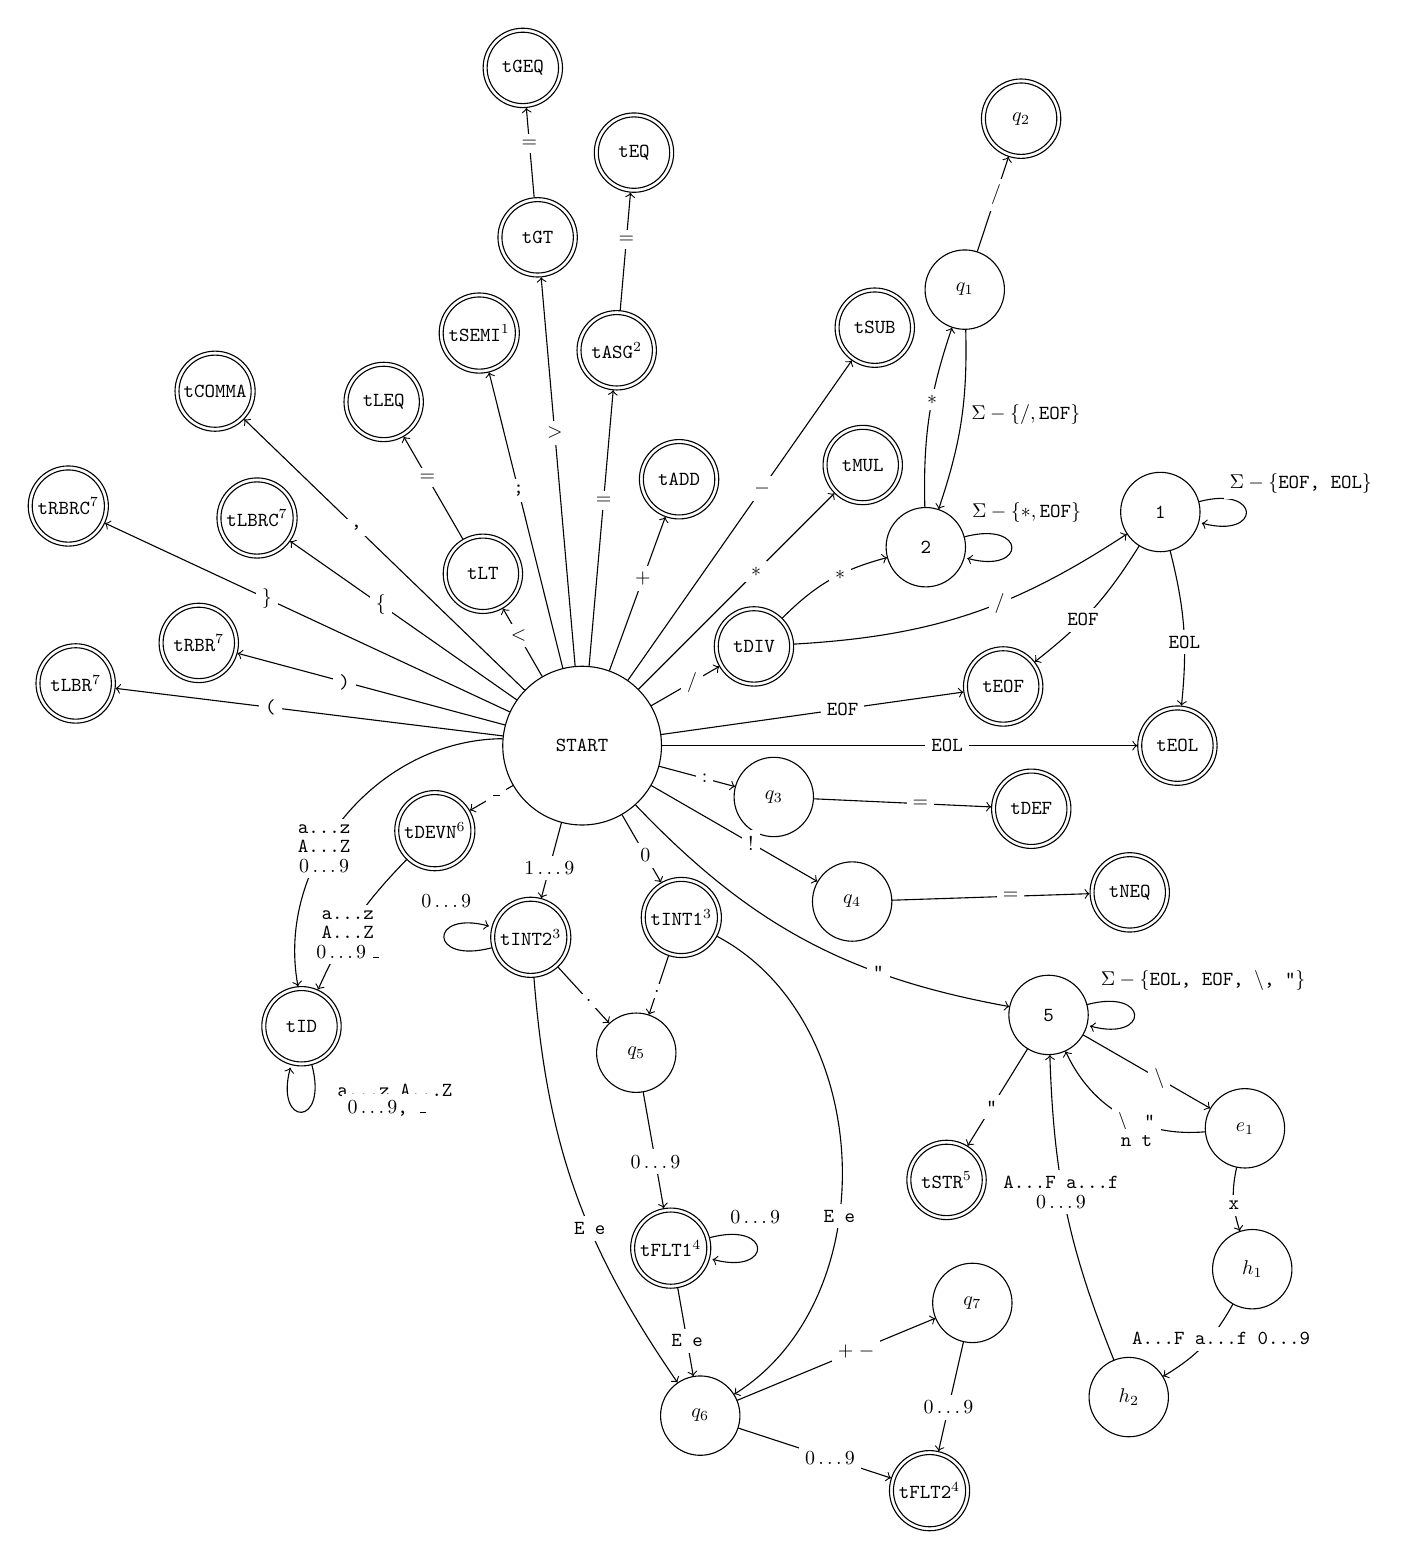
\begin{tikzpicture}[double distance=2pt, pos=0.6, state/.style={circle, draw, minimum size=1.4cm}, scale=0.72, every node/.style={transform shape}] 
        % START
        \node[state, minimum size=2.8cm] (start)   {\texttt{START}}; 

        % ; , 
        \node[state, accepting] (comma) at (136:9) {\texttt{tCOMMA}};
        \node[state, accepting] (semicolon) at (104:7.5) {\texttt{tSEMI$^1$}};
        % LT -> LEQ branch
        \node[state, accepting] (lt) at (120:3.5) {\texttt{tLT}};   
        \node[state, accepting] (leq) at (120:7) {\texttt{tLEQ}}; 

        % GT -> GEQ branch
        \node[state, accepting] (gt) at (95:9) {\texttt{tGT}};
        \node[state, accepting] (geq) at (95:12) {\texttt{tGEQ}}; 

        % ASSIGN -> EQ branch
        \node[state, accepting] (assign) at (85:7) {\texttt{tASG$^2$}}; 
        \node[state, accepting] (eq) at (85:10.5) {\texttt{tEQ}};
        
        % +, -, *
        \node[state, accepting] (plus) at (70:5) {\texttt{tADD}};
        \node[state, accepting] (minus) at (55:9) {\texttt{tSUB}};
        \node[state, accepting] (times) at (45:7) {\texttt{tMUL}};

        % /, komentare
        \node[state, accepting] (div) at (30:3.5) {\texttt{tDIV}};
        \node[state] (multicom) at (30:7) {\texttt{2}};
        \node[state] (linecom) at (22:11) {\texttt{1}};
        \node[state] (q1) at (50:10.5) {$q_1$};
        \node[state, accepting] (q2) at (55:13.5) {$q_2$};

        % eol, eof
        \node[state, accepting] (eof) at (8:7.5) {\texttt{tEOF}};
        \node[state, accepting] (eol) at (0:10.5) {\texttt{tEOL}};
       
        % def, neq
        \node[state] (q3) at (-15:3.5) {$q_3$};
        \node[state] (q4) at (-30:5.5) {$q_4$};
        \node[state, accepting] (def) at (-8:8) {\texttt{tDEF}};
        \node[state, accepting] (neq) at (-15:10) {\texttt{tNEQ}};

        
        % int, float
        \node[state, accepting] (zero) at (-60:3.5) {\texttt{tINT1$^3$}};
        \node[state, accepting] (int) at (-105:3.5) {\texttt{tINT2$^3$}};
        \node[state] (q5) at (-80:5.5) {$q_5$};
        \node[state, accepting] (float1) at (-80:9) {\texttt{tFLT1$^4$}};
        \node[state] (q6) at (-80:12) {$q_6$};
        \node[state] (q7) at (-55:12) {$q_7$};
        \node[state, accepting] (float2) at (-65:14.5) {\texttt{tFLT2$^4$}};

        % string
        \node[state] (beginstring) at (-30:9.5) {\texttt{5}};
        \node[state] (esc1) at (-30:13.5) {$e_1$};
        \node[state] (hex2) at (-50:15) {$h_2$};
        \node[state] (hex1) at (-38:15) {$h_1$};
        \node[state, accepting] (string) at (-50:10) {\texttt{tSTR$^5$}};

        %dev null, id
        \node[state, accepting] (devnull) at (210:3) {\texttt{tDEVN$^6$}};
        \node[state, accepting] (id) at (225:7) {\texttt{tID}};

        
        % brackets () and {}
        \node[state, accepting] (lbr) at (173:9) {\texttt{tLBR$^7$}};
        \node[state, accepting] (rbr) at (165:7) {\texttt{tRBR$^7$}};
        \node[state, accepting] (rcbr) at (155:10) {\texttt{tRBRC$^7$}};
        \node[state, accepting] (lcbr) at (145:7) {\texttt{tLBRC$^7$}};

    \path[->] 
        (start) edge node {\colorbox{white}{$<$}} (lt)
        (lt) edge node {\colorbox{white}{$=$}} (leq)

        (start) edge node {\colorbox{white}{$>$}} (gt)
        (gt) edge node {\colorbox{white}{$=$}} (geq)
        (start) edge node {\colorbox{white}{$=$}} (assign)
        (assign) edge node {\colorbox{white}{$=$}} (eq)
        (start) edge node {\colorbox{white}{$+$}} (plus)
        (start) edge node {\colorbox{white}{$-$}} (minus)
        (start) edge node {\colorbox{white}{$*$}} (times)

        (start) edge node {\colorbox{white}{$/$}} (div)
        (div) edge[bend right=15] node {\colorbox{white}{$/$}} (linecom)
        (div) edge[bend left=15] node {\colorbox{white}{$*$}} (multicom)
        (linecom) edge[in=120, out=60, loop right] node[above, xshift=1cm, yshift=0.2cm] {\colorbox{white}{$\Sigma-\{\texttt{EOF, EOL}\}$}} ()
        (start) edge node {\colorbox{white}{\texttt{EOF}}} (eof)
        (start) edge node {\colorbox{white}{\texttt{EOL}}} (eol)
        (linecom) edge[bend left=10] node {\colorbox{white}{\texttt{EOF}}} (eof)
        (linecom) edge[bend left=10] node {\colorbox{white}{\texttt{EOL}}} (eol)
        (multicom) edge[loop right] node[above, xshift=0.3cm, yshift=0.3cm] {\colorbox{white}{$\Sigma-\{*, \texttt{EOF}\}$}} ()
        (multicom) edge[bend left=10] node {\colorbox{white}{$*$}} (q1)
        (q1) edge[bend left=10] node[above right] {\colorbox{white}{$\Sigma-\{/, \texttt{EOF}\}$}} (multicom)
        (q1) edge node {\colorbox{white}{$/$}} (q2)
        (start) edge node {\colorbox{white}{$:$}} (q3)
        (start) edge node {\colorbox{white}{$!$}} (q4)
        (q3) edge node {\colorbox{white}{$=$}} (def)
        (q4) edge node {\colorbox{white}{$=$}} (neq)
        (start) edge node {\colorbox{white}{$1\dots9$}} (int)
        (int) edge[loop left] node[above, yshift=0.2cm]{\colorbox{white}{$0\dots9$}} ()
        (start) edge node {\colorbox{white}{$0$}} (zero)
        (int) edge node {\colorbox{white}{$.$}} (q5)
        (zero) edge node {\colorbox{white}{$.$}} (q5)
        (q5) edge node {\colorbox{white}{$0\dots9$}} (float1)
        (float1) edge[loop right] node[above, yshift=0.3cm] {\colorbox{white}{$0\dots9$}} ()
        (int) edge[bend right=15] node {\colorbox{white}{\texttt{E e}}} (q6)
        (zero) edge[bend left=60] node {\colorbox{white}{\texttt{E e}}} (q6)
        (float1) edge node {\colorbox{white}{\texttt{E e}}} (q6)
        (q6) edge node {\colorbox{white}{$0\dots9$}} (float2)
        (q6) edge node {\colorbox{white}{$+\;-$}} (q7)
        (q7) edge node {\colorbox{white}{$0\dots9$}} (float2)
        (start) edge[pos=0.7, bend right=18] node {\colorbox{white}{\texttt{"}}} (beginstring)
        (beginstring) edge node {\colorbox{white}{\texttt{\textbackslash}}} (esc1)
        
        (esc1) edge[bend left=35, pos=0.4] node {\colorbox{white}{\texttt{\textbackslash\; "}}} node[below] {\colorbox{white}{\texttt{n t}}} (beginstring)
        (esc1) edge[bend right=15] node {\colorbox{white}{\texttt{x}}} (hex1)
        (hex1) edge[bend left=15, pos=0.4] node[xshift=0.2cm] {\colorbox{white}{\texttt{A\dots F a\dots f 0\dots9}}} (hex2)
        (hex2) edge[bend left=10] node {\colorbox{white}{\texttt{A\dots F a\dots f}}} node[below] {\colorbox{white}{$0\dots9$}} (beginstring)
        (beginstring) edge[loop right] node[above, xshift=1.25cm, yshift=0.3cm] {\colorbox{white}{$\Sigma-\{$\texttt{EOL, EOF, \textbackslash, "\}}}} ()
        (beginstring) edge node {\colorbox{white}{\texttt{"}}} (string)

        (start) edge[pos=0.4] node {\colorbox{white}{\texttt{\_}}} (devnull) 
        (devnull) edge[bend right=10] node[above] {\colorbox{white}{\texttt{a\dots z}}} node {\colorbox{white}{\texttt{A\dots Z}}} node[below] {\colorbox{white}{\texttt{$0\dots9\;\_$}}} (id)
        (id) edge[loop below] node[above right, xshift=0.5cm] {\colorbox{white}{\texttt{a\dots z A\dots Z}}} node[below,yshift=0.4cm, xshift=1.6cm] {\colorbox{white}{\texttt{$0\dots9$, \_}}} ()
        (start) edge[bend right=50] node[above] {\colorbox{white}{\texttt{a\dots z}}} node {\colorbox{white}{\texttt{A\dots Z}}} node[below] {\colorbox{white}{\texttt{$0\dots9$}}} (id)

        (start) edge node {\colorbox{white}{\texttt{(}}} (lbr)
        (start) edge node {\colorbox{white}{\texttt{)}}} (rbr)
        (start) edge node {\colorbox{white}{\texttt{\{}}} (lcbr)
        (start) edge node {\colorbox{white}{\texttt{\}}}} (rcbr)

        (start) edge node {\colorbox{white}{\texttt{;}}} (semicolon)
        (start) edge node {\colorbox{white}{\texttt{,}}} (comma)
        ;
    \end{tikzpicture}
    \caption[DKA]{Deterministický konečný stavový automat$^8$}
    \label{KA}
\end{figure}
\footnotetext[1]{\texttt{tSEMI} změněno z \texttt{tSEMICOLON}}
\footnotetext[2]{\texttt{tASG} změněno z \texttt{tASSIGN}}
\footnotetext[3]{\texttt{tINT1} a \texttt{tINT2} obojí reprezentuje token \texttt{tINT}}
\footnotetext[4]{\texttt{tFLT1} a \texttt{tFLT2} obojí reprezentuje token \texttt{tFLOAT}}
\footnotetext[5]{\texttt{tSTR} změněno z \texttt{tSTRING}}
\footnotetext[6]{\texttt{tDEVN} změněno z \texttt{tDEVNULL}}
\footnotetext[7]{\texttt{tLBR} změněno z \texttt{tLBRACKET}, obdobně pro \texttt{tRBR}, \texttt{tLBRC} změněno z \texttt{tLBRACE}}
\footnotetext[8]{$\Sigma$ reprezentuje ASCII hodnoty větší než 32 včetně a ASCII hodnoty 10, 13 a \texttt{EOF}}
\newpage
    \section{LL gramatika}
    \begin{figure}[h!]
        \begin{Verbatim}[fontsize=\relsize{-0.5}]
<START>         ->  package main EOL <SCEL> 
<SCEL>          ->  func <PROG> EOL <SCEL>
<SCEL>          ->  EOL <SCEL>
<SCEL>          ->  EOF
<PROG>          ->  id ( <PARAMS_DEF> ) <RET> { <BODY> }
<BODY>          ->  eps
<BODY>          ->  return <VALUE_EXTRA>
<BODY>          ->  EOL <BODY>
<BODY>          ->  if <IF> EOL <BODY>
<BODY>          ->  for <FOR> EOL <BODY>
<BODY>          ->  id <ID> EOL <BODY>
<ID>            ->  ( <PARAMS> )
<ID>            ->  := <EXPR_TYPE>
<ID>            ->  <ID_MORE> = <ID_ASSIGN>
<ID_MORE>       ->  eps
<ID_MORE>       ->  , id <ID_MORE>  
<EXPR_TYPE>     ->  <TYPE>
<EXPR_TYPE>     ->  <EXPR>
<EXPR_TYPE_M>   ->  eps
<EXPR_TYPE_M>   ->  , <EXPR_TYPE> <EXPR_TYPE_M>
<TYPE>          ->  id
<TYPE>          ->  INTEGER_VAL
<TYPE>          ->  FLOAT_VAL
<TYPE>          ->  STRING_VAL
<VALUE_EXTRA>   ->  <EXPR_TYPE> <EXPR_TYPE_M>
<ID_ASSIGN>     ->  <VALUE_EXTRA>
<ID_ASSIGN>     ->  id ( <PARAMS> )
<DATA_TYPE>     ->  int
<DATA_TYPE>     ->  string
<DATA_TYPE>     ->  float64
<PARAMS>        ->  eps
<PARAMS>        ->  <TYPE> <TYPE_MORE>
<TYPE_MORE>     ->  eps
<TYPE_MORE>     ->  , <TYPE> <TYPE_MORE>
<PARAMS_DEF>    ->  eps
<PARAMS_DEF>    ->  id <DATA_TYPE> <PARAMS_DEF_M> 
<PARAMS_DEF_M>  ->  eps
<PARAMS_DEF_M>  ->  , id <DATA_TYPE> <PARAMS_DEF_M>
<RET>           ->  eps
<RET>           ->  ( <RET_BODY> )
<RET_BODY>      ->  eps
<RET_BODY>      ->  <DATA_TYPE> <RET_BODY_M>
<RET_BODY_M>    ->  eps
<RET_BODY_M>    ->  , <DATA_TYPE> <RET_BODY_M>
<IF>            ->  <EXPR> { <BODY> } else { <BODY> }
<FOR>           ->  <EXPR_TYPE> ; <EXPR> ; <EXPR> { <BODY> }
        \end{Verbatim}
        \caption{LL gramatika}
    \end{figure}
    \label{gramatika}
    
    \newpage
    \section{LL tabulka}
        \begin{figure}[h!]
            \begin{adjustbox}{scale=0.65,angle=90,center}
                \begin{tabular}{| c |  c | c | c | c | c | c | c | c | c | c | c | c | c | c | c | c | c | c | c | c | c | c | c |}\hline
                    &\texttt{package main} & \texttt{EOL} & \texttt{EOF} & \texttt{func} & \texttt{id} & \texttt{(} & \texttt{)} & \texttt{\{} & \texttt{\}} & \texttt{return} & \texttt{if} & \texttt{for} & \texttt{:=} & \texttt{=} & \texttt{,} & \texttt{INTEGER\_VAL} & \texttt{FLOAT\_VAL} & \texttt{STRING\_VAL} & \texttt{int} & \texttt{string} & \texttt{float64} & \texttt{;} & \texttt{\$} \\\hline
                   \texttt{<START>}         & 1  &    &    &    &    &    &    &    &    &    &    &    &    &    &    &    &    &    &    &    &    & & \\\hline
                   \texttt{<SCEL>}          &    & 3  &  4 &  2 &    &    &    &    &    &    &    &    &    &    &    &    &    &    &    &    &    & &  \\\hline
                   \texttt{<PROG>}          &    &    &    &    &  5 &    &    &    &    &    &    &    &    &    &    &    &    &    &    &    &    & &  \\\hline
                   \texttt{<BODY>}          &    & 8  &    &    & 11 &    &    &    &  6 & 7  & 9  & 10 &    &    &    &    &    &    &    &    &    & & 6 \\\hline
                   \texttt{<ID>}            &    &    &    &    &    & 12 &    &    &    &    &    &    & 13 &    & 14 &    &    &    &    &    &    & &  \\\hline
                   \texttt{<ID\_MORE>}      &    &    &    &    &    &    &    &    &    &    &    &    &    & 15 & 16 &    &    &    &    &    &    & & 15 \\\hline
                   \texttt{<EXPR\_TYPE>}    &    &    &    &    & 17 &    &    &    &    &    &    &    &    &    &    & 17 & 17 & 17 &    &    &    & &  \\\hline
                   \texttt{<EXPR\_TYPE\_M>} &    & 19 &    &    &    &    &    &    & 19 &    &    &    &    &    & 20 &    &    &    &    &    &    & & 19 \\\hline
                   \texttt{<TYPE>}          &    &    &    &    & 21 &    &    &    &    &    &    &    &    &    &    & 22 & 23 & 24 &    &    &    & &  \\\hline
                   \texttt{<VALUE\_EXTRA>}  &    &    &    &    & 25 &    &    &    &    &    &    &    &    &    &    & 25 & 25 & 25 &    &    &    & &  \\\hline
                   \texttt{<ID\_ASSIGN>}    &    &    &    &    & 27 &    &    &    &    &    &    &    &    &    &    & 26 & 26 & 26 &    &    &    & &  \\\hline
                   \texttt{<DATA\_TYPE>}    &    &    &    &    &    &    &    &    &    &    &    &    &    &    &    &    &    &    & 28 & 29 & 30 & &  \\\hline
                   \texttt{<PARAMS>}        &    &    &    &    & 32 &    & 31 &    &    &    &    &    &    &    &    & 32 & 32 & 32 &    &    &    & & 31 \\\hline
                   \texttt{<TYPE\_MORE>}    &    &    &    &    &    &    & 33 &    &    &    &    &    &    &    & 34 &    &    &    &    &    &    & & 33 \\\hline
                   \texttt{<PARAMS\_DEF>}   &    &    &    &    & 36 &    & 35 &    &    &    &    &    &    &    &    &    &    &    &    &    &    & & 35 \\\hline
                   \texttt{<PARAMS\_DEF\_M>}&    &    &    &    &    &    & 37 &    &    &    &    &    &    &    & 38 &    &    &    &    &    &    & & 37 \\\hline
                   \texttt{<RET>}           &    &    &    &    &    & 40 &    & 39 &    &    &    &    &    &    &    &    &    &    &    &    &    & & 39 \\\hline
                   \texttt{<RET\_BODY>}     &    &    &    &    &    &    & 41 &    &    &    &    &    &    &    &    &    &    &    & 42 & 42 & 42 & & 41 \\\hline
                   \texttt{<RET\_BODY\_M>}  &    &    &    &    &    &    & 43 &    &    &    &    &    &    &    & 44 &    &    &    &    &    &    & & 43 \\\hline
                   \texttt{<IF>}            &    &    &    &    &    &    &    &    &    &    &    &    &    &    &    &    &    &    &    &    &    & &  \\\hline
                   \texttt{<FOR>}           &    &    &    &    & 46 &    &    &    &    &    &    &    &    &    &    & 46 & 46 & 46 &    &    &    & &  \\\hline
                \end{tabular}
            \end{adjustbox}
            \label{lltabulka}
            \caption{LL tabulka}
        \end{figure}


\newpage
        \bibliographystyle{czechiso}
        \renewcommand{\refname}{Zdroje}
        \bibliography{ifj}
\end{document}